% Options for packages loaded elsewhere
\PassOptionsToPackage{unicode}{hyperref}
\PassOptionsToPackage{hyphens}{url}
%
\documentclass[
]{article}
\usepackage{lmodern}
\usepackage{amsmath}
\usepackage{ifxetex,ifluatex}
\ifnum 0\ifxetex 1\fi\ifluatex 1\fi=0 % if pdftex
  \usepackage[T1]{fontenc}
  \usepackage[utf8]{inputenc}
  \usepackage{textcomp} % provide euro and other symbols
  \usepackage{amssymb}
\else % if luatex or xetex
  \usepackage{unicode-math}
  \defaultfontfeatures{Scale=MatchLowercase}
  \defaultfontfeatures[\rmfamily]{Ligatures=TeX,Scale=1}
\fi
% Use upquote if available, for straight quotes in verbatim environments
\IfFileExists{upquote.sty}{\usepackage{upquote}}{}
\IfFileExists{microtype.sty}{% use microtype if available
  \usepackage[]{microtype}
  \UseMicrotypeSet[protrusion]{basicmath} % disable protrusion for tt fonts
}{}
\makeatletter
\@ifundefined{KOMAClassName}{% if non-KOMA class
  \IfFileExists{parskip.sty}{%
    \usepackage{parskip}
  }{% else
    \setlength{\parindent}{0pt}
    \setlength{\parskip}{6pt plus 2pt minus 1pt}}
}{% if KOMA class
  \KOMAoptions{parskip=half}}
\makeatother
\usepackage{xcolor}
\IfFileExists{xurl.sty}{\usepackage{xurl}}{} % add URL line breaks if available
\IfFileExists{bookmark.sty}{\usepackage{bookmark}}{\usepackage{hyperref}}
\hypersetup{
  pdftitle={Distribuição Normal},
  pdfauthor={Prof.~André Luiz Cunha},
  hidelinks,
  pdfcreator={LaTeX via pandoc}}
\urlstyle{same} % disable monospaced font for URLs
\usepackage[margin=1in]{geometry}
\usepackage{color}
\usepackage{fancyvrb}
\newcommand{\VerbBar}{|}
\newcommand{\VERB}{\Verb[commandchars=\\\{\}]}
\DefineVerbatimEnvironment{Highlighting}{Verbatim}{commandchars=\\\{\}}
% Add ',fontsize=\small' for more characters per line
\usepackage{framed}
\definecolor{shadecolor}{RGB}{248,248,248}
\newenvironment{Shaded}{\begin{snugshade}}{\end{snugshade}}
\newcommand{\AlertTok}[1]{\textcolor[rgb]{0.94,0.16,0.16}{#1}}
\newcommand{\AnnotationTok}[1]{\textcolor[rgb]{0.56,0.35,0.01}{\textbf{\textit{#1}}}}
\newcommand{\AttributeTok}[1]{\textcolor[rgb]{0.77,0.63,0.00}{#1}}
\newcommand{\BaseNTok}[1]{\textcolor[rgb]{0.00,0.00,0.81}{#1}}
\newcommand{\BuiltInTok}[1]{#1}
\newcommand{\CharTok}[1]{\textcolor[rgb]{0.31,0.60,0.02}{#1}}
\newcommand{\CommentTok}[1]{\textcolor[rgb]{0.56,0.35,0.01}{\textit{#1}}}
\newcommand{\CommentVarTok}[1]{\textcolor[rgb]{0.56,0.35,0.01}{\textbf{\textit{#1}}}}
\newcommand{\ConstantTok}[1]{\textcolor[rgb]{0.00,0.00,0.00}{#1}}
\newcommand{\ControlFlowTok}[1]{\textcolor[rgb]{0.13,0.29,0.53}{\textbf{#1}}}
\newcommand{\DataTypeTok}[1]{\textcolor[rgb]{0.13,0.29,0.53}{#1}}
\newcommand{\DecValTok}[1]{\textcolor[rgb]{0.00,0.00,0.81}{#1}}
\newcommand{\DocumentationTok}[1]{\textcolor[rgb]{0.56,0.35,0.01}{\textbf{\textit{#1}}}}
\newcommand{\ErrorTok}[1]{\textcolor[rgb]{0.64,0.00,0.00}{\textbf{#1}}}
\newcommand{\ExtensionTok}[1]{#1}
\newcommand{\FloatTok}[1]{\textcolor[rgb]{0.00,0.00,0.81}{#1}}
\newcommand{\FunctionTok}[1]{\textcolor[rgb]{0.00,0.00,0.00}{#1}}
\newcommand{\ImportTok}[1]{#1}
\newcommand{\InformationTok}[1]{\textcolor[rgb]{0.56,0.35,0.01}{\textbf{\textit{#1}}}}
\newcommand{\KeywordTok}[1]{\textcolor[rgb]{0.13,0.29,0.53}{\textbf{#1}}}
\newcommand{\NormalTok}[1]{#1}
\newcommand{\OperatorTok}[1]{\textcolor[rgb]{0.81,0.36,0.00}{\textbf{#1}}}
\newcommand{\OtherTok}[1]{\textcolor[rgb]{0.56,0.35,0.01}{#1}}
\newcommand{\PreprocessorTok}[1]{\textcolor[rgb]{0.56,0.35,0.01}{\textit{#1}}}
\newcommand{\RegionMarkerTok}[1]{#1}
\newcommand{\SpecialCharTok}[1]{\textcolor[rgb]{0.00,0.00,0.00}{#1}}
\newcommand{\SpecialStringTok}[1]{\textcolor[rgb]{0.31,0.60,0.02}{#1}}
\newcommand{\StringTok}[1]{\textcolor[rgb]{0.31,0.60,0.02}{#1}}
\newcommand{\VariableTok}[1]{\textcolor[rgb]{0.00,0.00,0.00}{#1}}
\newcommand{\VerbatimStringTok}[1]{\textcolor[rgb]{0.31,0.60,0.02}{#1}}
\newcommand{\WarningTok}[1]{\textcolor[rgb]{0.56,0.35,0.01}{\textbf{\textit{#1}}}}
\usepackage{graphicx}
\makeatletter
\def\maxwidth{\ifdim\Gin@nat@width>\linewidth\linewidth\else\Gin@nat@width\fi}
\def\maxheight{\ifdim\Gin@nat@height>\textheight\textheight\else\Gin@nat@height\fi}
\makeatother
% Scale images if necessary, so that they will not overflow the page
% margins by default, and it is still possible to overwrite the defaults
% using explicit options in \includegraphics[width, height, ...]{}
\setkeys{Gin}{width=\maxwidth,height=\maxheight,keepaspectratio}
% Set default figure placement to htbp
\makeatletter
\def\fps@figure{htbp}
\makeatother
\setlength{\emergencystretch}{3em} % prevent overfull lines
\providecommand{\tightlist}{%
  \setlength{\itemsep}{0pt}\setlength{\parskip}{0pt}}
\setcounter{secnumdepth}{5}
\ifluatex
  \usepackage{selnolig}  % disable illegal ligatures
\fi

\title{Distribuição Normal}
\usepackage{etoolbox}
\makeatletter
\providecommand{\subtitle}[1]{% add subtitle to \maketitle
  \apptocmd{\@title}{\par {\large #1 \par}}{}{}
}
\makeatother
\subtitle{Aula 2}
\author{Prof.~André Luiz Cunha}
\date{21/05/2021}

\begin{document}
\maketitle

\hypertarget{transformauxe7uxe3o-de-escala}{%
\section{Transformação de escala}\label{transformauxe7uxe3o-de-escala}}

Um passo importante de qualquer análise de dados é a uniformização do
intervalo de dados, de modo que todas as variáveis do banco de dados
tenham o mesmo intervalo de variação. Na literatura temos dois tipos de
transformação

\begin{Shaded}
\begin{Highlighting}[]
\CommentTok{\# Conjunto de valores aleatórios com média 50 e desvio 15.}
\NormalTok{(x }\OtherTok{\textless{}{-}} \FunctionTok{rnorm}\NormalTok{(}\DecValTok{100}\NormalTok{, }\DecValTok{50}\NormalTok{, }\DecValTok{15}\NormalTok{))}
\end{Highlighting}
\end{Shaded}

\begin{verbatim}
##   [1] 81.95492 63.70145 59.84402 29.03614 36.83837 52.31954 47.48039 16.96690
##   [9] 79.02751 42.22281 49.93790 72.16353 32.75996 62.75825 62.04287 34.34612
##  [17] 56.74150 22.51613 38.40618 41.54669 46.13155 35.90177 62.68782 56.70538
##  [25] 64.97357 47.59002 51.65478 63.96517 39.68162 31.25627 88.35457 19.24039
##  [33] 58.89939 61.81595 34.87505 68.15630 34.21176 47.18986 63.18132 36.26722
##  [41] 47.71326 56.51160 66.98419 49.05309 64.77358 45.82890 62.42944 43.79950
##  [49] 26.60777 54.16811 76.10061 44.60954 60.52618 15.77870 65.35911 96.65488
##  [57] 53.61846 54.65751 38.53526 82.34462 52.68212 60.41166 69.38666 46.06130
##  [65] 47.40419 61.44111 40.32041 51.39102 78.02165 59.96898 50.18075 54.75996
##  [73] 81.92924 45.55012 42.18383 62.26823 62.06747 70.70899 29.05432 38.32979
##  [81] 59.46730 31.51399 43.59235 47.96043 40.52407 35.08822 43.51377 40.17733
##  [89] 43.41403 84.55618 45.04116 40.96168 59.59239 38.38171 49.40163 40.94027
##  [97] 59.01125 47.68123 50.32989 52.94093
\end{verbatim}

\begin{Shaded}
\begin{Highlighting}[]
\FunctionTok{summary}\NormalTok{(x)}
\end{Highlighting}
\end{Shaded}

\begin{verbatim}
##    Min. 1st Qu.  Median    Mean 3rd Qu.    Max. 
##   15.78   40.84   50.06   51.60   62.05   96.65
\end{verbatim}

\hypertarget{normalizauxe7uxe3o-01}{%
\subsection{Normalização {[}0,1{]}}\label{normalizauxe7uxe3o-01}}

\begin{Shaded}
\begin{Highlighting}[]
\NormalTok{x\_norm }\OtherTok{\textless{}{-}}\NormalTok{ (x }\SpecialCharTok{{-}} \FunctionTok{min}\NormalTok{(x)) }\SpecialCharTok{/}\NormalTok{ (}\FunctionTok{max}\NormalTok{(x) }\SpecialCharTok{{-}} \FunctionTok{min}\NormalTok{(x))}
\FunctionTok{summary}\NormalTok{(x\_norm)}
\end{Highlighting}
\end{Shaded}

\begin{verbatim}
##    Min. 1st Qu.  Median    Mean 3rd Qu.    Max. 
##  0.0000  0.3098  0.4239  0.4429  0.5721  1.0000
\end{verbatim}

\hypertarget{padronizar--33}{%
\subsection{Padronizar {[}-3,3{]}}\label{padronizar--33}}

\begin{Shaded}
\begin{Highlighting}[]
\NormalTok{x\_pad }\OtherTok{\textless{}{-}}\NormalTok{ (x }\SpecialCharTok{{-}} \FunctionTok{mean}\NormalTok{(x)) }\SpecialCharTok{/} \FunctionTok{sd}\NormalTok{(x)}
\FunctionTok{summary}\NormalTok{(x\_pad)}
\end{Highlighting}
\end{Shaded}

\begin{verbatim}
##     Min.  1st Qu.   Median     Mean  3rd Qu.     Max. 
## -2.26265 -0.67973 -0.09709  0.00000  0.66033  2.84644
\end{verbatim}

A padronização dos dados nada mais é do que a transformação para a
escala da curva normal padrão (z-padrão). Vide Figura 1 a tabela
z-padrão.

\begin{figure}
\centering
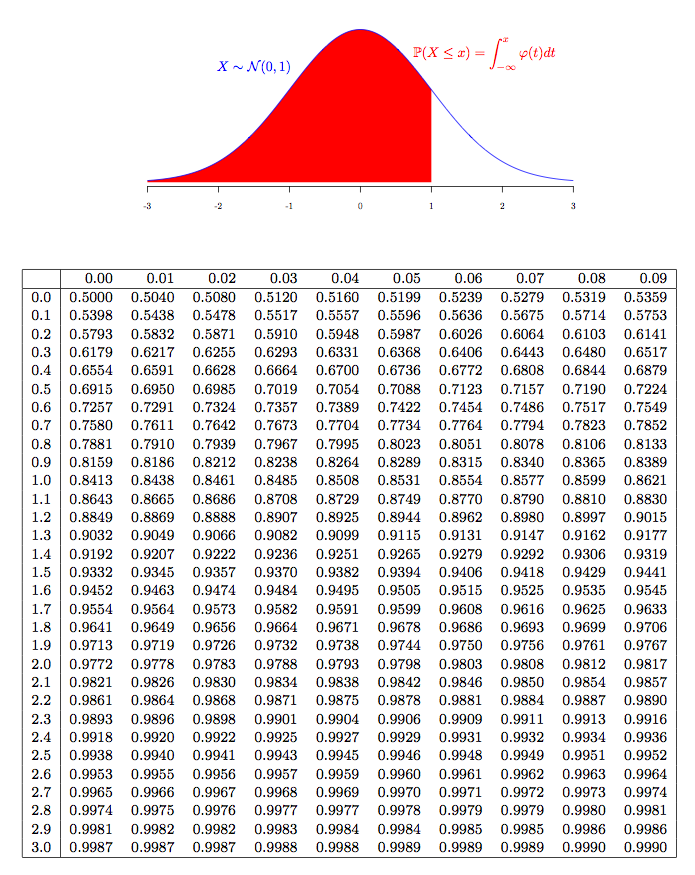
\includegraphics{normal-table.png}
\caption{Tabela Z-padrão}
\end{figure}

\begin{Shaded}
\begin{Highlighting}[]
\DocumentationTok{\#\# OLHANDO A TABELA}
\CommentTok{\#z = 1,0 {-}{-}{-}{-}\textgreater{} p(z) = 0,1587}
\DecValTok{1} \SpecialCharTok{{-}} \DecValTok{2} \SpecialCharTok{*} \FloatTok{0.1587}
\end{Highlighting}
\end{Shaded}

\begin{verbatim}
## [1] 0.6826
\end{verbatim}

\begin{Shaded}
\begin{Highlighting}[]
\CommentTok{\#z = 2,0 {-}{-}{-}{-}\textgreater{} p(z) = 0,0228}
\DecValTok{1} \SpecialCharTok{{-}} \DecValTok{2} \SpecialCharTok{*} \FloatTok{0.0228}
\end{Highlighting}
\end{Shaded}

\begin{verbatim}
## [1] 0.9544
\end{verbatim}

\begin{Shaded}
\begin{Highlighting}[]
\CommentTok{\# p(z) = 95\% {-}{-}{-}{-}{-}\textgreater{} z(p = 0,025) = ?}
\FloatTok{1.96}
\end{Highlighting}
\end{Shaded}

\begin{verbatim}
## [1] 1.96
\end{verbatim}

\begin{Shaded}
\begin{Highlighting}[]
\CommentTok{\# p(z) = 99\% {-}{-}{-}{-}{-}\textgreater{} z =??}
\FloatTok{2.575}
\end{Highlighting}
\end{Shaded}

\begin{verbatim}
## [1] 2.575
\end{verbatim}

\hypertarget{funuxe7uxf5es-do-r}{%
\section{Funções do R}\label{funuxe7uxf5es-do-r}}

\hypertarget{nuxfameros-aleatuxf3rios}{%
\subsection{Números aleatórios}\label{nuxfameros-aleatuxf3rios}}

\begin{Shaded}
\begin{Highlighting}[]
\DocumentationTok{\#\# Uniformemente distribuídos}
\end{Highlighting}
\end{Shaded}

Função: \texttt{runif(n,\ min,\ max)}

\begin{Shaded}
\begin{Highlighting}[]
\FunctionTok{runif}\NormalTok{(}\DecValTok{10}\NormalTok{)}
\end{Highlighting}
\end{Shaded}

\begin{verbatim}
##  [1] 0.7446925 0.5346661 0.5412608 0.4029396 0.9155983 0.5955964 0.5216851
##  [8] 0.0957525 0.4979599 0.4498968
\end{verbatim}

\begin{Shaded}
\begin{Highlighting}[]
\FunctionTok{runif}\NormalTok{(}\DecValTok{10}\NormalTok{, }\DecValTok{100}\NormalTok{, }\DecValTok{150}\NormalTok{)}
\end{Highlighting}
\end{Shaded}

\begin{verbatim}
##  [1] 108.4437 120.4169 133.6860 123.8815 128.2571 121.4598 101.1226 111.9532
##  [9] 128.4889 106.8365
\end{verbatim}

\begin{Shaded}
\begin{Highlighting}[]
\DocumentationTok{\#\# Normalmente distribuídos}
\end{Highlighting}
\end{Shaded}

Função: \texttt{rnorm(n,\ mean,\ sd)}

\begin{Shaded}
\begin{Highlighting}[]
\FunctionTok{rnorm}\NormalTok{(}\DecValTok{10}\NormalTok{)}
\end{Highlighting}
\end{Shaded}

\begin{verbatim}
##  [1]  0.519541457 -0.637647229 -0.446732105 -0.428468526  0.009846958
##  [6]  1.320150538  0.015717242 -1.107154262 -0.846468565 -0.956322799
\end{verbatim}

\begin{Shaded}
\begin{Highlighting}[]
\FunctionTok{rnorm}\NormalTok{(}\DecValTok{10}\NormalTok{, }\DecValTok{100}\NormalTok{, }\DecValTok{15}\NormalTok{)}
\end{Highlighting}
\end{Shaded}

\begin{verbatim}
##  [1]  87.81023 100.38945 100.87788 115.11102 116.57867 125.59136 102.83233
##  [8] 130.02110 100.60110 112.35421
\end{verbatim}

\hypertarget{distribuiuxe7uxe3o-normal}{%
\subsection{Distribuição Normal}\label{distribuiuxe7uxe3o-normal}}

Encontrando o valor z-padrão com a função
\texttt{qnorm(area\ da\ curva,\ mean=0,\ sd=1)}

\begin{itemize}
\tightlist
\item
  Unicaudal a esquerda: \(z_\alpha = qnorm(\alpha)\)
\item
  Unicaudal a direita: \(z_\alpha = qnorm(1 - \alpha)\)
\item
  Bicaudal: \(z_frac{\alpha}{2} = qnorm(1 - \alpha/2)\)
\end{itemize}

\begin{Shaded}
\begin{Highlighting}[]
\FunctionTok{qnorm}\NormalTok{(.}\DecValTok{90}\NormalTok{)}
\end{Highlighting}
\end{Shaded}

\begin{verbatim}
## [1] 1.281552
\end{verbatim}

\begin{Shaded}
\begin{Highlighting}[]
\FunctionTok{qnorm}\NormalTok{(.}\DecValTok{5}\NormalTok{)}
\end{Highlighting}
\end{Shaded}

\begin{verbatim}
## [1] 0
\end{verbatim}

Encontrando o p-valor com a função
\texttt{pnorm(valor\ z,\ mean=0,\ sd=1)}

\begin{itemize}
\tightlist
\item
  Unicaudal a esquerda: \(p-value = pnorm(z, lower.tail=TRUE)\)
\item
  Unicaudal a direita: \(p-value = pnorm(z, lower.tail=FALSE)\)
\item
  Bicaudal: \(p-value = 2 * pnorm(abs(z), lower.tail=FALSE)\)
\end{itemize}

\begin{Shaded}
\begin{Highlighting}[]
\FunctionTok{pnorm}\NormalTok{(}\FloatTok{1.96}\NormalTok{)}
\end{Highlighting}
\end{Shaded}

\begin{verbatim}
## [1] 0.9750021
\end{verbatim}

\begin{Shaded}
\begin{Highlighting}[]
\FunctionTok{pnorm}\NormalTok{(}\FloatTok{1.96}\NormalTok{, }\AttributeTok{lower.tail =} \ConstantTok{FALSE}\NormalTok{)}
\end{Highlighting}
\end{Shaded}

\begin{verbatim}
## [1] 0.0249979
\end{verbatim}

\begin{Shaded}
\begin{Highlighting}[]
\FunctionTok{pnorm}\NormalTok{(}\DecValTok{0}\NormalTok{)}
\end{Highlighting}
\end{Shaded}

\begin{verbatim}
## [1] 0.5
\end{verbatim}

Encontrando a densidade do valor com a função
\texttt{dnorm(valor\ z,\ mean=0,\ sd=1)}

\begin{Shaded}
\begin{Highlighting}[]
\FunctionTok{dnorm}\NormalTok{(}\FloatTok{1.96}\NormalTok{)}
\end{Highlighting}
\end{Shaded}

\begin{verbatim}
## [1] 0.05844094
\end{verbatim}

\begin{Shaded}
\begin{Highlighting}[]
\FunctionTok{dnorm}\NormalTok{(}\SpecialCharTok{{-}}\FloatTok{1.96}\NormalTok{)}
\end{Highlighting}
\end{Shaded}

\begin{verbatim}
## [1] 0.05844094
\end{verbatim}

\begin{Shaded}
\begin{Highlighting}[]
\FunctionTok{dnorm}\NormalTok{(}\DecValTok{0}\NormalTok{)}
\end{Highlighting}
\end{Shaded}

\begin{verbatim}
## [1] 0.3989423
\end{verbatim}

\textbf{EXEMPLO 1}

\begin{Shaded}
\begin{Highlighting}[]
\DocumentationTok{\#\# P(z \textgreater{} 1,65)}
\FunctionTok{pnorm}\NormalTok{(}\FloatTok{1.65}\NormalTok{, }\AttributeTok{lower.tail =} \ConstantTok{FALSE}\NormalTok{)}
\end{Highlighting}
\end{Shaded}

\begin{verbatim}
## [1] 0.04947147
\end{verbatim}

\begin{Shaded}
\begin{Highlighting}[]
\DocumentationTok{\#\# P(z \textless{} 1,65)}
\FunctionTok{pnorm}\NormalTok{(}\FloatTok{1.65}\NormalTok{)}
\end{Highlighting}
\end{Shaded}

\begin{verbatim}
## [1] 0.9505285
\end{verbatim}

\begin{Shaded}
\begin{Highlighting}[]
\DocumentationTok{\#\# P(1,40 \textless{} z \textless{} 1,70)}
\FunctionTok{pnorm}\NormalTok{(}\FloatTok{1.7}\NormalTok{) }\SpecialCharTok{{-}} \FunctionTok{pnorm}\NormalTok{(}\FloatTok{1.4}\NormalTok{)}
\end{Highlighting}
\end{Shaded}

\begin{verbatim}
## [1] 0.0361912
\end{verbatim}

\hypertarget{histogramas}{%
\subsection{Histogramas}\label{histogramas}}

\begin{Shaded}
\begin{Highlighting}[]
\FunctionTok{hist}\NormalTok{(}\FunctionTok{runif}\NormalTok{(}\DecValTok{10000}\NormalTok{))}
\end{Highlighting}
\end{Shaded}

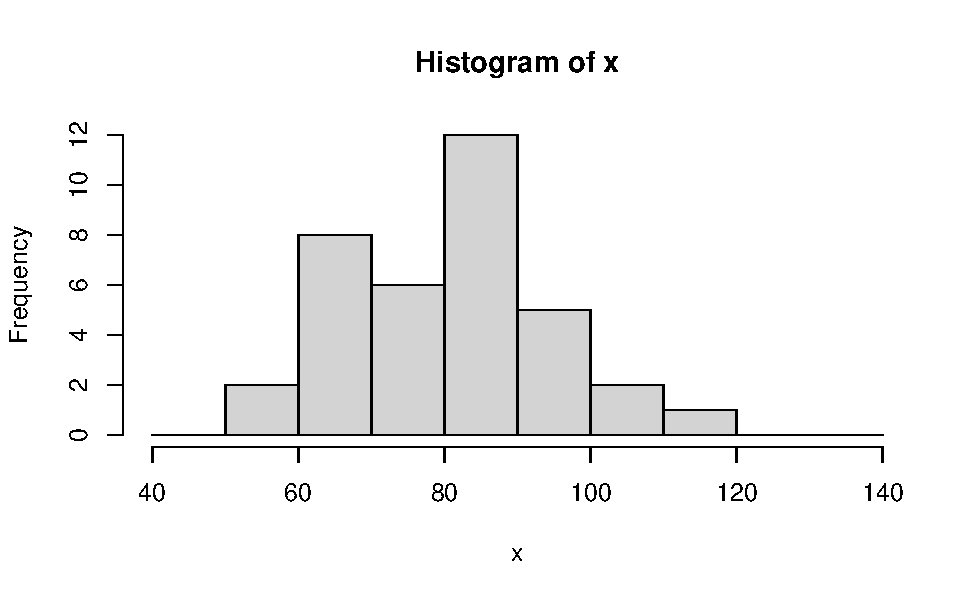
\includegraphics{DistNormal_files/figure-latex/unnamed-chunk-12-1.pdf}

\begin{Shaded}
\begin{Highlighting}[]
\FunctionTok{hist}\NormalTok{(}\FunctionTok{rnorm}\NormalTok{(}\DecValTok{10000}\NormalTok{), }\AttributeTok{breaks =} \FunctionTok{seq}\NormalTok{(}\SpecialCharTok{{-}}\DecValTok{5}\NormalTok{,}\DecValTok{5}\NormalTok{,.}\DecValTok{1}\NormalTok{),}
     \AttributeTok{freq =} \ConstantTok{FALSE}\NormalTok{)}
\end{Highlighting}
\end{Shaded}

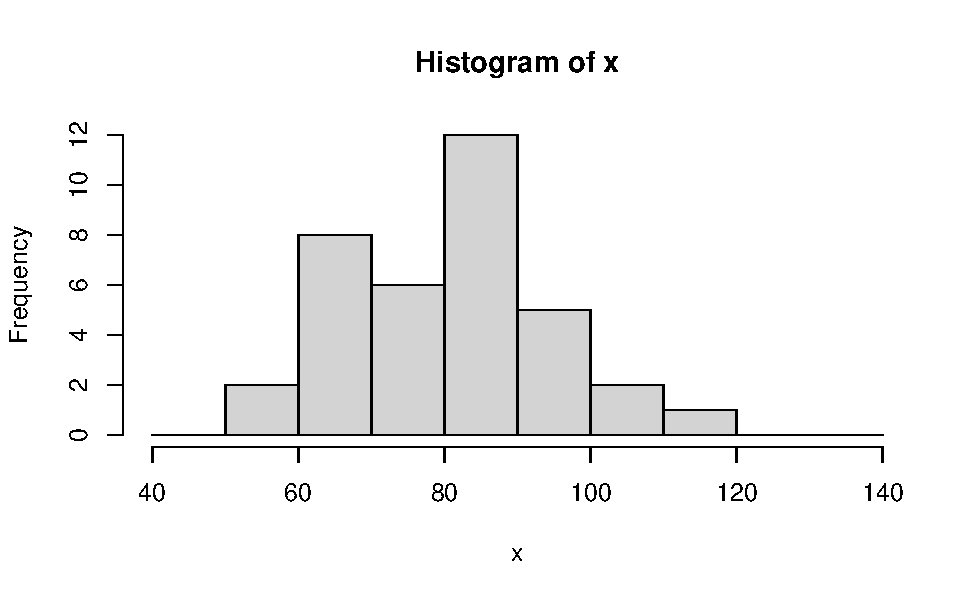
\includegraphics{DistNormal_files/figure-latex/unnamed-chunk-13-1.pdf}

\textbf{EXEMPLO 2}

\begin{Shaded}
\begin{Highlighting}[]
\NormalTok{x }\OtherTok{=} \FunctionTok{c}\NormalTok{(}\DecValTok{58}\NormalTok{,}\DecValTok{78}\NormalTok{,}\DecValTok{84}\NormalTok{,}\DecValTok{90}\NormalTok{,}\DecValTok{97}\NormalTok{,}\DecValTok{70}\NormalTok{,}
      \DecValTok{90}\NormalTok{,}\DecValTok{86}\NormalTok{,}\DecValTok{82}\NormalTok{,}\DecValTok{59}\NormalTok{,}\DecValTok{90}\NormalTok{,}\DecValTok{70}\NormalTok{,}
      \DecValTok{74}\NormalTok{,}\DecValTok{83}\NormalTok{,}\DecValTok{90}\NormalTok{,}\DecValTok{75}\NormalTok{,}\DecValTok{88}\NormalTok{,}\DecValTok{84}\NormalTok{,}
      \DecValTok{68}\NormalTok{,}\DecValTok{96}\NormalTok{,}\DecValTok{70}\NormalTok{,}\DecValTok{94}\NormalTok{,}\DecValTok{70}\NormalTok{,}\DecValTok{110}\NormalTok{,}
      \DecValTok{67}\NormalTok{,}\DecValTok{68}\NormalTok{,}\DecValTok{75}\NormalTok{,}\DecValTok{80}\NormalTok{,}\DecValTok{68}\NormalTok{,}\DecValTok{82}\NormalTok{,}
      \DecValTok{104}\NormalTok{,}\DecValTok{92}\NormalTok{,}\DecValTok{112}\NormalTok{,}\DecValTok{84}\NormalTok{,}\DecValTok{98}\NormalTok{,}\DecValTok{80}\NormalTok{)}


\DocumentationTok{\#\# Análise descritiva}
\FunctionTok{summary}\NormalTok{(x)}
\end{Highlighting}
\end{Shaded}

\begin{verbatim}
##    Min. 1st Qu.  Median    Mean 3rd Qu.    Max. 
##   58.00   70.00   82.50   82.39   90.00  112.00
\end{verbatim}

\begin{Shaded}
\begin{Highlighting}[]
\NormalTok{hdados }\OtherTok{\textless{}{-}} \FunctionTok{hist}\NormalTok{(x, }
               \AttributeTok{breaks =} \FunctionTok{seq}\NormalTok{(}\DecValTok{40}\NormalTok{,}\DecValTok{140}\NormalTok{,}\DecValTok{10}\NormalTok{))}
\end{Highlighting}
\end{Shaded}

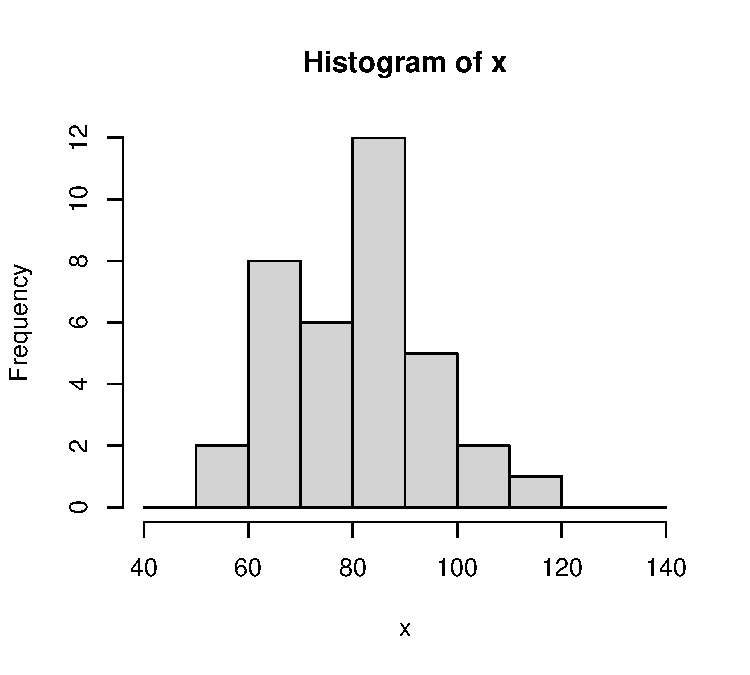
\includegraphics{DistNormal_files/figure-latex/unnamed-chunk-15-1.pdf}

\begin{Shaded}
\begin{Highlighting}[]
\NormalTok{hdados}\SpecialCharTok{$}\NormalTok{breaks}
\end{Highlighting}
\end{Shaded}

\begin{verbatim}
##  [1]  40  50  60  70  80  90 100 110 120 130 140
\end{verbatim}

\begin{Shaded}
\begin{Highlighting}[]
\NormalTok{hdados}\SpecialCharTok{$}\NormalTok{counts}
\end{Highlighting}
\end{Shaded}

\begin{verbatim}
##  [1]  0  2  8  6 12  5  2  1  0  0
\end{verbatim}

\begin{Shaded}
\begin{Highlighting}[]
\NormalTok{hdados}\SpecialCharTok{$}\NormalTok{density}
\end{Highlighting}
\end{Shaded}

\begin{verbatim}
##  [1] 0.000000000 0.005555556 0.022222222 0.016666667 0.033333333 0.013888889
##  [7] 0.005555556 0.002777778 0.000000000 0.000000000
\end{verbatim}

O parâmetro \texttt{density} traz a razão entre a porcentagem de
elementos e o intervalo de bins, tanto que a soma das porcentagens
\texttt{density} é igual a\\
\texttt{0.1}

\begin{Shaded}
\begin{Highlighting}[]
\CommentTok{\#. }

\FunctionTok{sum}\NormalTok{(hdados}\SpecialCharTok{$}\NormalTok{density)}
\end{Highlighting}
\end{Shaded}

\begin{verbatim}
## [1] 0.1
\end{verbatim}

Ao multiplicar cada densidade pelo intervalo do bin, a porcentagem total
será de 100\%.

\begin{Shaded}
\begin{Highlighting}[]
\FunctionTok{sum}\NormalTok{(hdados}\SpecialCharTok{$}\NormalTok{density) }\SpecialCharTok{*} \DecValTok{10}
\end{Highlighting}
\end{Shaded}

\begin{verbatim}
## [1] 1
\end{verbatim}

\hypertarget{testes-do-r}{%
\section{Testes do R}\label{testes-do-r}}

\begin{Shaded}
\begin{Highlighting}[]
\NormalTok{x\_pad }\OtherTok{\textless{}{-}}\NormalTok{ (x }\SpecialCharTok{{-}} \FunctionTok{mean}\NormalTok{(x))}\SpecialCharTok{/}\FunctionTok{sd}\NormalTok{(x)}
\end{Highlighting}
\end{Shaded}

\hypertarget{qui-quadrado}{%
\subsection{Qui-quadrado}\label{qui-quadrado}}

\begin{Shaded}
\begin{Highlighting}[]
\FunctionTok{chisq.test}\NormalTok{(x, }\FunctionTok{rnorm}\NormalTok{(}\DecValTok{36}\NormalTok{, }\FunctionTok{mean}\NormalTok{(x), }\FunctionTok{sd}\NormalTok{(x)) )}
\end{Highlighting}
\end{Shaded}

\begin{verbatim}
## Warning in chisq.test(x, rnorm(36, mean(x), sd(x))): Chi-squared approximation
## may be incorrect
\end{verbatim}

\begin{verbatim}
## 
##  Pearson's Chi-squared test
## 
## data:  x and rnorm(36, mean(x), sd(x))
## X-squared = 792, df = 770, p-value = 0.2836
\end{verbatim}

\hypertarget{kolomogorv-smirnof}{%
\subsection{Kolomogorv-Smirnof}\label{kolomogorv-smirnof}}

\begin{Shaded}
\begin{Highlighting}[]
\FunctionTok{ks.test}\NormalTok{(x, }\StringTok{"pnorm"}\NormalTok{, }\FunctionTok{mean}\NormalTok{(x), }\FunctionTok{sd}\NormalTok{(x))}
\end{Highlighting}
\end{Shaded}

\begin{verbatim}
## Warning in ks.test(x, "pnorm", mean(x), sd(x)): ties should not be present for
## the Kolmogorov-Smirnov test
\end{verbatim}

\begin{verbatim}
## 
##  One-sample Kolmogorov-Smirnov test
## 
## data:  x
## D = 0.10407, p-value = 0.8304
## alternative hypothesis: two-sided
\end{verbatim}

\begin{Shaded}
\begin{Highlighting}[]
\FunctionTok{ks.test}\NormalTok{(x\_pad, }\StringTok{"pnorm"}\NormalTok{)}
\end{Highlighting}
\end{Shaded}

\begin{verbatim}
## Warning in ks.test(x_pad, "pnorm"): ties should not be present for the
## Kolmogorov-Smirnov test
\end{verbatim}

\begin{verbatim}
## 
##  One-sample Kolmogorov-Smirnov test
## 
## data:  x_pad
## D = 0.10407, p-value = 0.8304
## alternative hypothesis: two-sided
\end{verbatim}

\hypertarget{shapiro}{%
\subsection{Shapiro}\label{shapiro}}

\begin{Shaded}
\begin{Highlighting}[]
\FunctionTok{shapiro.test}\NormalTok{(x)}
\end{Highlighting}
\end{Shaded}

\begin{verbatim}
## 
##  Shapiro-Wilk normality test
## 
## data:  x
## W = 0.97612, p-value = 0.6139
\end{verbatim}

\end{document}
